\documentclass[a4paper,11pt]{report}

\usepackage[latin1]{inputenc}
\usepackage{amsmath}
\usepackage{amsfonts}
\usepackage{amssymb}
\usepackage{graphicx}
\usepackage[spanish]{babel}
\usepackage{fancyhdr}
\usepackage{indentfirst}
\usepackage{verbatim}
\usepackage{alltt}
\usepackage{hyperref}
\usepackage[left=3cm,top=3cm,right=2.5cm,bottom=2.5cm]{geometry}

% style for code citation
\newenvironment{code}
	{\begin{quote}\begin{alltt}}
	{\end{alltt}\end{quote}}

% fast commands to write system components names
\newcommand{\plfs}{\textit{plfs }}
\newcommand{\kplfs}{\textit{kplfs }}
\newcommand{\uplfs}{\textit{uplfs }}
\newcommand{\dpld}{\textit{dpld }}
\newcommand{\pldb}{\textit{pldb }}
\newcommand{\umcc}{\textit{umcc }}
\newcommand{\umc}{\textit{umc }}
\newcommand{\umcr}{\textit{umcr }}
\newcommand{\dplc}{\textit{dplc }}
\newcommand{\famon}{\textit{fam }}

% 4 levels of enumeration and indexing
\setcounter{secnumdepth}{4}
\setcounter{tocdepth}{4}

% Title Page
\author{
  Jonathan Mart� Fraiz \\
  \textit{jonathan.marti@upc.edu}
  \and
  Llu�s Vilanova Garc�a \\
  \textit{xscript@gmx.net}
}

\title{
  \textbf{
  Desplegamiento Paralelitzado \\
  de Aplicaciones en PlanetLab \\
  a Trav�s del Sistema de Ficheros
  }
}


\begin{document}

\maketitle

\tableofcontents

% Headers
\pagestyle{fancy}
%\fancyhf{} % delete all adjustments
% From here on, fancyhead is used to configure the header, fancyfoot for the
% footer
% Justification: C=centered, R=right, L=left, (nothing)=LRC
% Page: O=odd, E=even, (nothing)=OE
\fancyhead[]{}  % chapter number
\fancyhead[L]{\leftmark}  % chapter number
%\fancyhead[R]{\thepage} % page number
% Modifies the width of the header and footer lines
\renewcommand{\chaptermark}[1]{
	\markboth{\chaptername\  \thechapter. #1}{}
}
\renewcommand{\headrulewidth}{0.4pt}

\chapter{Qu� y porqu� lo queremos hacer?}

Tanto la documentaci�n como la implementaci�n se encuentran disponibles en la
p�gina del proyecto \cite{PLFS}.

Cabe notar que, como inicialmente nos centraremos en las operaciones de
desplegamiento, siempre que nos refiramos a \plfs, s�lo estaremos haciendo
referencia, realmente, al subconjunto dedicado al desplegamiento.

El proyecto pretende juntar b�sicamente dos conceptos con tal de conseguir dos
grandes objetivos:



\section{Facilidad de uso}

A trav�s de una interf�cie que todo el mundo ya conozca y necesite un m�nimo
de aprendizaje y permita un f�cil desarrollo de aplicaciones de m�s alto
nivel.

Este objetivo pretende conseguirse a trav�s de la implementaci�n de un sistema
de ficheros, con una estructura a�n por determinar, pero que permita desplegar
una aplicaci�n de una forma tan f�cil como copiar un fichero en un directorio
concreto, evento que disparar�a el sistema de distribuci�n de ficheros.



\section{Eficiencia en la transferencia de ficheros}

Como la aplicaci�n a desplegar necesita ser copiada a todos los nodos de un
slice, no basta con copiarla directamente a un sistema de ficheros "en red"
convencional, puesto que se enviar�a a un punto central y luego todos los
nodos, al arrancar el servicio, leer�an a la vez el programa para poder
ponerlo en marcha, saturando innecesariamente la red.

Para �ste fin, la idea de una distribuci�n multicast es ideal, ya que
permitir�a ahorrar al m�ximo el ancho de banda, permitiendo un desplegamiento
en paralelo y evitando al m�ximo las aglomeraciones de datos innecesarias.

Como la mayor�a de routers de Internet no soportan el enrutamiento multicast,
es por eso que har�a falta un servicio en modo usuario que se encargara de
hacer �sta distribuci�n.


\chapter{Arquitectura del sistema}

\textbf{\textit{En este cap�tulo comentamos la arquitectura general del
sistema, los componentes necesarios, el sistema de ficheros y las operaciones
que debe implementar.}}



\section{Componentes}

En este apartado mostraremos un esquema inicial de los principales
componentes que necesitar�a el sistema presentado (figura
\ref{fig:arquitectura}):

\begin{description}
	\item [\kplfs:] PlanetLab File System (Kernel-mode Side)\\
		Componente del sistema de ficheros para PlanetLab que funciona dentro
		del n�cleo de Linux.
		\\
		Este componente, puede en realidad ser varios, cada uno dando
		unos servicios concretos (uno para el desplegamiento, uno para
		monitorizaci�n, \ldots).

	\item [\uplfs:] PlanetLab File System (User-mode Side)\\
		Componente del sistema de ficheros para PlanetLab que funciona en modo
		usuario.
		\\
		Este componente en realidad hace de intermediario entre el
		propio sistema de ficheros (es decir, el n�cleo) y los
		componentes que permiten realizar las funcionalidades y
		comunicaciones (en nuestro caso, ser�a \dpld).

	\item [\dpld:] Deployer Daemon\\
		Componente encargado de mandar las �rdenes de desplegamiento y
		mantener actualizada la visi�n que tiene el usuario sobre los
		slices de desplegamiento.

	\item [\pldb :] PlanetLab Data Base (para obtener inicialmente la lista
		de nodos de un slice)\\
		Componente para obtener datos de PlanetLab Central (PLC).

	\item [\umcc :] User-mode Multicast Client\\
		Componente encargado de las comunicaciones entre un sistema cualquiera
		y la red multicast.

	\item [\umcr :] User-mode Multicast Router\\
		Componente encargado de enrutar paquetes multicast.

	\item [\dplc :] Deployer Client\\
		Componente encargado de desplegar los ficheros en un nodo e informar
		de los slices que tiene creados.

	\item [\famon:] File Alteration Monitor\\
		Componente encargado de vigilar qu� ficheros cambian en un nodo.
\end{description}

\begin{figure}[h]
	\centering
	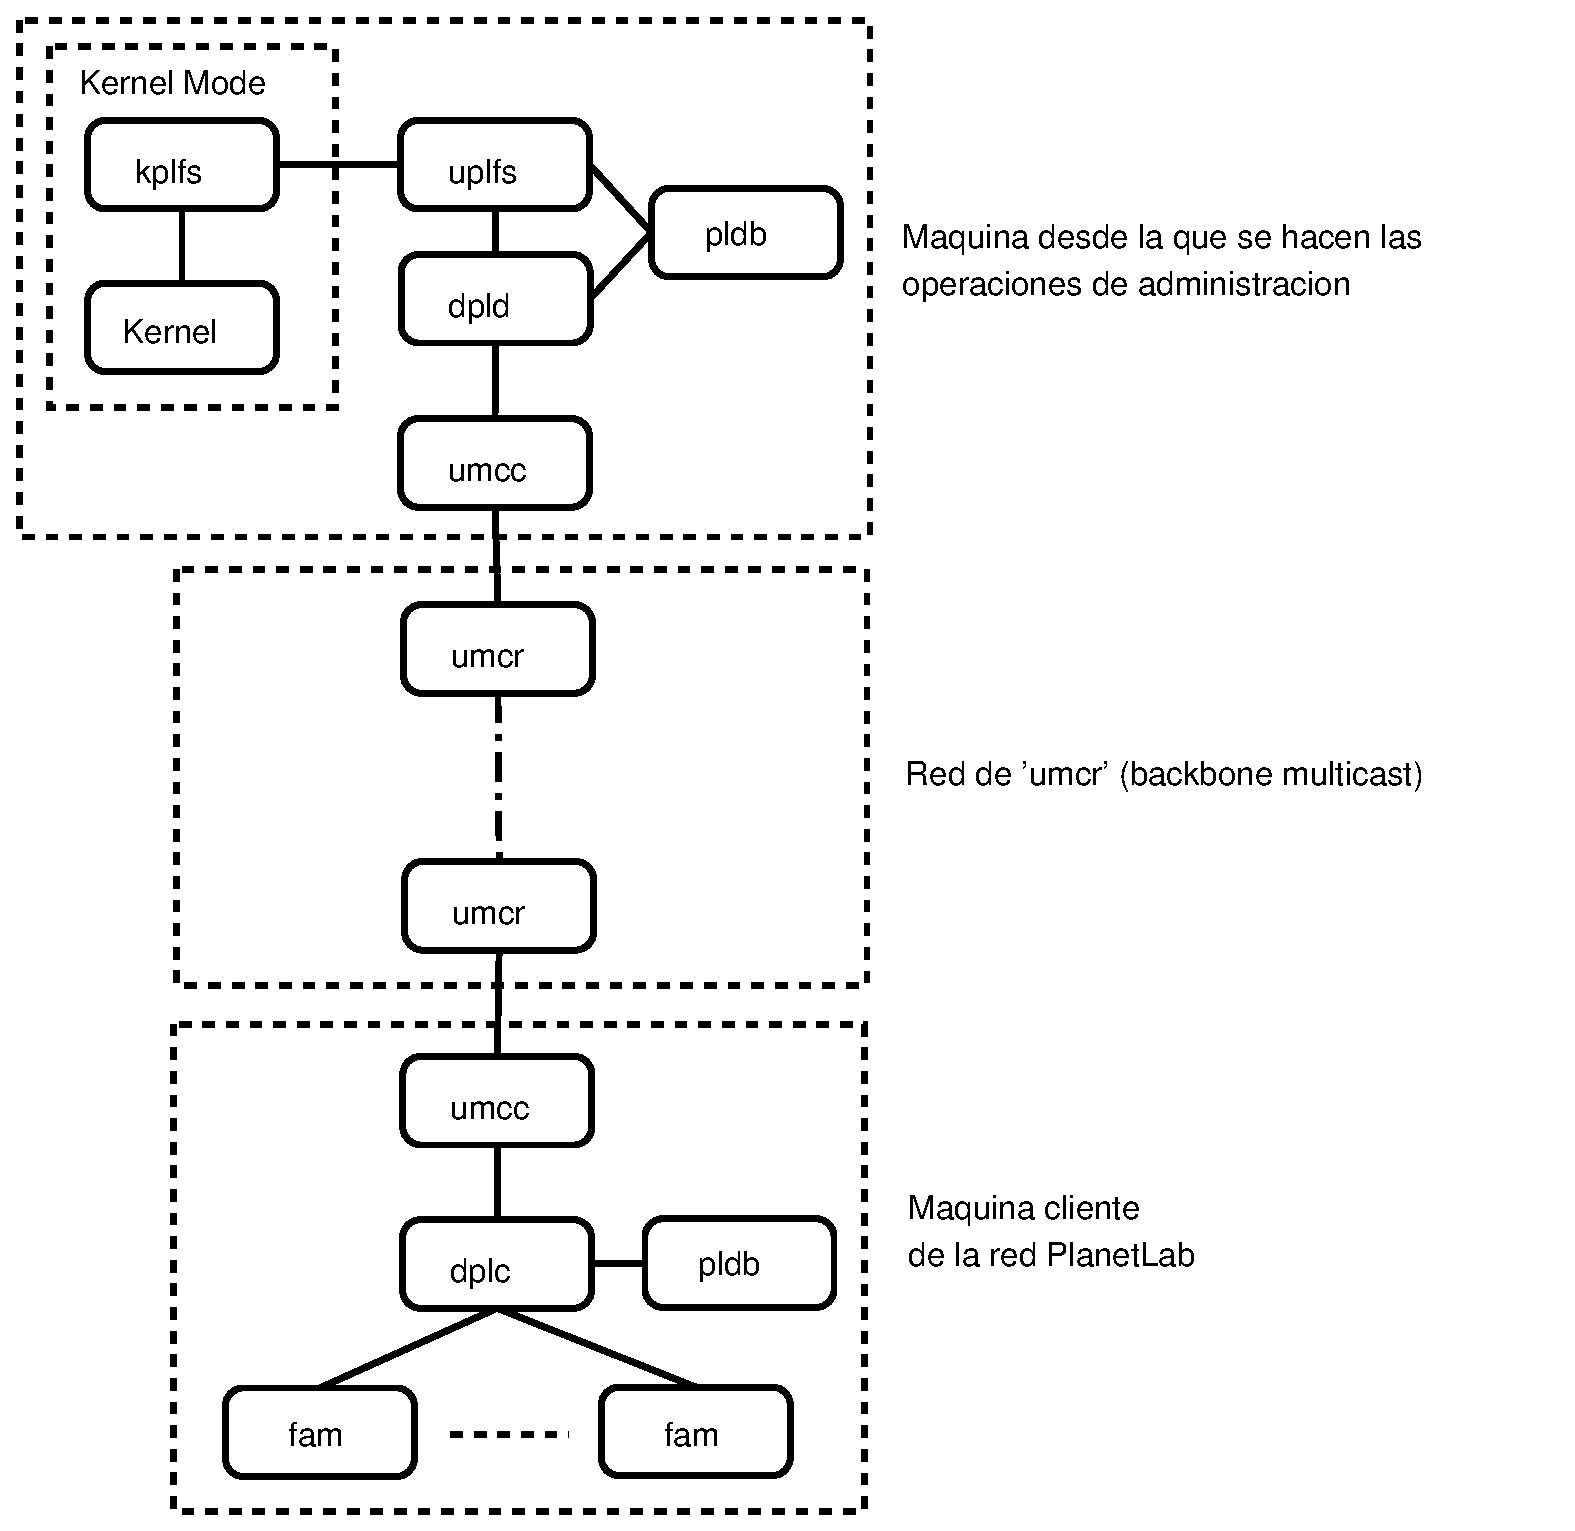
\includegraphics[scale=0.5]{arquitectura.eps}
	\caption{Arquitectura del Sistema}
	\label{fig:arquitectura}
\end{figure}



\section{L�gica del sistema}

El sistema, adem�s de las funcionalidades propias de despliegue de
aplicaciones, debe poder realizar las siguientes operaciones para poder saber
como llegar y a d�nde puede llegar. Es decir, debe poder conseguir la
informaci�n necesaria sobre los slices disponibles en PlanetLab y sus nodos, y
por otra parte, debe poder descubrir su punto de entrada a la red multicast
desde el exterior.

De modo que el sistema debe permitir:

\begin{itemize}
	\item Descubrimiento de slices en PlanetLab \\
		Al acceder al sistema de ficheros (\kplfs-\uplfs), hay que preguntar a
		un servicio de PlanetLab si existe o no un slice dado (al hacer un
		move de un ejectuable a un directorio que es un slice) o cu�les
		existen (al hacer un ls para ver los slices disponibles).

		Para ello, hace falta encontrar el nodo con el servicio de PlanetLab
		de BD \textbf{m�s cercano} (por ahora solo hay uno, y es
		\textit{PlanetLab Central}) y preguntarle:
		\begin{itemize}
			\item si existe un slice concreto

			\item qu� slices hay
		\end{itemize}

	\item Descubrimiento de nodos en PlanetLab \\
		Como en el caso anterior, nos hace falta preguntar a PlanetLab por los
		nodos, tanto a nivel general, como por los asociados a un slice.

	\item Descubrimiento del nodo de entrada a la red de distribuci�n
		multicast.
\end{itemize}

Con tal de minimizar la latencia y ocupaci�n innecesaria del ancho de banda,
para todos los anteriores puntos hace falta encontrar el nodo \textbf{m�s
cercano} que da un servicio concreto.

Para ello, se podr�a utilizar un servicio DNS al estilo Akamai, tal como
utiliza google, o algo como CoDNS \cite{CoDNS}, subproyecto de Codeen
\cite{Codeen}, que nos dan la IP del nodo m�s cercano que proporciona un
servicio conreto.



\section{Esquema de \plfs (PlanetLab File System)}

Antes de comentar el esquema del �rbol de ficheros y directorios de \plfs, es
necesario dejar bien claro que hemos dise�ado el sistema con la idea de
permitir una cierta flexibilidad al usuario y que pueda diferenciar entre dos
tipos de ficheros:

\begin{description}
	\item [Los ficheros que se despliegan como shared]:\\
		Que todos los nodos del slice destino tendr�n por igual, bajo la
		condici�n que adem�s deben de ser inmutables (ej: el programa
		principal de la aplicaci�n).

	\item [Los ficheros que se despliegan como unshared]:\\
		Que ser�n propios de cada nodo (ej: cada nodo podr�a asumir un
		rol distinto si tuviera ficheros de configuraci�n propios).
\end{description}

Como veremos ahora, y durante todo el documento, esta idea es b�sica para el
dise�o que planteamos, puesto que en varios puntos el comportamiento del
sistema depender� del tipo de ficheros que estemos tratando.

Dicho lo cual, pasamos a presentar el esquema del �rbol de directorios y
ficheros como se puede apreciar en la figura:

\begin{code}
	/plfs
	|-slices
	| `-<slice>
	|   |-backup
	|   |-key
	|   |-passwd
	|   |-script
	|   |-nodes
	|   | `-<node>
	|   |   `-unshared
	|   `-shared
	`-nodes
	  `-<node>
	    `-slices
	      `-<slice> -> /plfs/slices/<slice>
\end{code}

A continuaci�n una explicaci�n de los diferentes ficheros y directorios:

\begin{description}
	\item[\texttt{/plfs/slices/\textless{}slice\textgreater/backup}] :\\
		Este fichero contiene una URI que indica el repositorio central
		de backup donde se puedan encontrar los ficheros \texttt{shared}
		en su versi�n original (ver el apartado 2.x sobre Redespliegue).

	\item[\texttt{/plfs/slices/\textless{}slice\textgreater/key}] :\\
		Este fichero contiene la clave privada ssh correspondiente al
		slice.

	\item[\texttt{/plfs/slices/\textless{}slice\textgreater/passwd}] :\\
		Este fichero contiene el password asociado a la clave privada
		del slice.

	\item[\texttt{/plfs/slices/\textless{}slice\textgreater/script}] :\\
		�ste fichero es un shell script que se ejecutar� en cada m�quina una
		vez hecho el desplegamiento.
		\\
		El script tiene un s�lo par�metro que puede ser:

		% TODO(~): NOTA MENTAL: �al terminar la m�quina virtual, ya
		% ejecutar� dicho startup->stop?
		\begin{description}
			\item [start:] lleva a cabo las operaciones para
				arrancar el servicio desplegado

			\item [stop:] lleva a cabo las operaciones para parar
				el servicio

			\item [deploy:] lleva a cabo las operaciones necesarias
				para preparar el arranque del servicio
		\end{description}

	\item[\texttt{/plfs/slices/\textless{}slice\textgreater/nodes/\textless{}node\textgreater/unshared}] :\\
		�ste directorio es propio de cada nodo en el contexto del slice que
		estamos mirando; puede servir para guardar ficheros de configuraci�n
		espec�ficos de cada m�quina, sin hacer nunca un desplegamiento al
		grupo entero.

	\item[\texttt{/plfs/slices/\textless{}slice\textgreater/shared}] :\\
		�ste directorio contiene los ficheros de los que se hace un
		desplegamiento al grupo entero (slice). La condici�n que deben
		cumplir los contenidos de �ste directorio, es que sean
		inmutables de cara a \plfs.
\end{description}

Tal como est� hecho el esquema, permitir�a que alguien pusiera un directorio
de administraci�n en, por ejemplo,
\texttt{/plfs/slices/\textless{}slice\textgreater/monitor} con estad�sticas de
funcionamiento del slice, u otro
\texttt{/plfs/nodes/\textless{}node\textgreater/monitor} con estad�sticas de
funcionamiento de un nodo concreto.



\section{Operaciones de \plfs}

Las posibles operaciones que \plfs permite, y por ende, que \kplfs implemente
y puede llegar a comunicar a \uplfs, son las propias de un sistema de
ficheros, es decir (seg�n las operaciones que puede realizar un usuario desde
la l�nea de comandos):

\begin{description}
	\item [\texttt{ls}] :\\
		Operaciones de consulta de contenido de directorios y/o
		propiedades.

		\begin{itemize}
			\item Listado de slices (v�a m�dulo \pldb)

			\item Listado de nodos (v�a m�dulo \pldb)

			\item Listado de ficheros desplegados (\texttt{shared}
				y \texttt{unshared}).
		\end{itemize}

	\item [\texttt{mv}] :\\
		Lo que nosotros implementaremos ser� un \textit{move} de ficheros
		(aplicaci�n a desplegar) a un slice (conjunto de nodos, representado
		por el directorio
		\texttt{/plfs/slices/\textless{slice\textgreater/shared}}) o nodo
		concreto (representado por el directorio
		\texttt{/plfs/slices/\textless{slice\textgreater/nodes/\textless{}node\textgreater/unshared}}).
		Es decir, \textbf{NO} permitiremos operaciones como:

		\begin{itemize}
			\item mover nodos

			\item mover slices

			\item \ldots
		\end{itemize}

	\item [\texttt{cp}] :\\
		Igual que en un \textit{move}, pero copiando los ficheros de or�gen.

	\item [\textit{edici�n}] :\\
		La edici�n de un fichero provocar� el redespliegue del mismo
		una vez sea cerrado.
		%TODO \cite (ver apartado 2.x sobre Redespliegue)

	\item [\textit{lectura}] :\\
		La lectura de un fichero provocar� su importaci�n previa en
		caso de no estar cacheado.

	\item [\texttt{rename}] :\\
		Soportado solo para ficheros y directorios que cuelgan de
		\texttt{shared} o \texttt{unshared}.

	\item [\texttt{rm}] :\\
		Soportado solo para ficheros y directorios que cuelgan de
		\texttt{shared} o \texttt{unshared}.

	\item [\texttt{mkdir}] :\\
		Seg�n en que directorio se haga, las implicaciones son
		distintas:

		\begin{itemize}
			\item En \texttt{/plfs/slices}: Crea un slice sin nodos asociados

			\item En \texttt{/plfs/slices/\textless{}slice\textgreater/nodes}:
				A�ade un nodo a un slice

			\item En \texttt{/plfs/nodes}: A�ade un nodo al sistema
				PlanetLab

			\item En los directorios \texttt{shared} y
				\texttt{unshared} crea �se directorio, seg�n
				corresponda
		\end{itemize}

		Los tres primeros puntos, como no entran dentro del
		desplegamiento de aplicaciones, no han sido pensados en
		profundidad para llevarlos a cabo.

	\item [\texttt{rmdir}] :\\
		Igual que en el caso anterior, seg�n en que directorio se haga, las
		implicaciones son distintas:

		\begin{itemize}
			\item En \texttt{/plfs/slices}: Elimina un slice de PlanetLab

			\item En \texttt{/plfs/slices/\textless{}slice\textgreater/nodes}:
				Elimina un nodo de un slice

			\item En \texttt{/plfs/nodes}: Elimina un nodo del sistema
				PlanetLab

			\item En los directorios \texttt{shared} y
				\texttt{unshared} elimina el directorio que
				corresponda.
		\end{itemize}

		De nuevo, los tres primeros puntos, como no entran dentro del
		desplegamiento de aplicaciones, no han sido pensados en
		profundidad para llevarlos a cabo.

	\item [\texttt{touch}] :\\
		\textbf{NO} soportado.

	\item[\texttt{chown}, \texttt{chmod}] :\\
		\textbf{NO} soportado.

	\item[\texttt{ln}] :\\
		\textbf{NO} soportado.

	\item[Otras operaciones] :\\
		\textbf{NO} soportadas.
\end{description}



\section{L�gica de Desplegamiento}

Despu�s de pensar diferentes posibilidades sobre como el usuario podr�a llevar
a cabo realmente el despliegue mediante el sistema de ficheros, hemos llegado
a la conclusi�n de que el usuario deber� realizar los siguientes pasos:

\begin{enumerate}
	\item 
		El usuario realiza \texttt{mv/cp} de los ficheros que
		desea desplegar, y estos son transmitidos mediante el proceso de
		despliegue que a continuaci�n comentamos.

	\item 
		A continuaci�n el usuario realiza \texttt{mv/cp} del script de
		arranque de despliegue, que tambi�n es desplegado mediante el
		mismo proceso hacia los nodos destino.
\end{enumerate}

Adem�s, y como es obvio dada la naturaleza del propio sistema de ficheros, se
deber� cumplir la siguiente precondici�n antes de poder realizar el despliegue:

\textit{Precondici�n}: El slice destino est� ya creado (ej: \texttt{mkdir}).

Una vez aclarado lo anterior, pasamos a describir como se realizar�a de forma
general el despliegue de los ficheros a trav�s de los diferentes componentes
del sistema:

\begin{enumerate}
	\item \kplfs $\rightarrow$ \uplfs \\
		Se informa de los ficheros de aplicaci�n a desplegar i del slice
		o nodo destino (en el caso de ser un solo nodo el
		destino, la comunicaci� se establece directamente
		desde \uplfs hacia \dplc).

	\item \uplfs $\rightarrow$ \dpld \\
		\uplfs redirige el mensaje al componente indicado por este (\dpld),
		puesto que \kplfs puede manejar la vista de diferentes componentes.

	\item \dpld $\rightarrow$ \umcc \\
		Se comunica el slice destino, se dan los ficheros a desplegar y el
		shell script con los comandos a ejecutar una vez desplegados.

	\item \umcc $\rightarrow$ red \umcr \\
		Se inyectan los paquetes a enviar con destino a un grupo en la
		red \umc.\\
		En nuestro caso, el grupo destino ser�a un slice y el
		desplegamiento se realizar� a aquellos nodos donde haya \dplc,
		de modo que ser�n siempre conocidos por la red multicast.

	\item intra-red \umcr (red multicast) \\
		Los nodos de la red \umcr encaminan el conjunto de paquetes
		hacia el grupo multicast de destino.\\
		En nuestro caso encaminar�n los ficheros, script, etc de
		la aplicaci�n a desplegar hacia los nodos de \dplc que forman
		parte del slice destino.

	\item red \umcr $\rightarrow$ \umcc \\
		Los paquetes llegan finalmente a los nodos que conforman el
		grupo destino multicast.
		En nuestro caso, los ficheros, script, etc. llegan finalmente a
		los nodos destino y son procesados por el m�dulo \umcc.

	\item \umcc $\rightarrow$ \dplc \\
		El m�dulo \umcc hace llegar los paquetes a desplegar al \dplc.

	\item \dplc $\rightarrow$ slice destino (ssh) \\
		Se despliega la aplicaci�n (se copian los ficheros), y una vez hecho
		esto, se ejecuta el shell script adjuntado, en caso de estar
		presente. Para ello, primero ejecuta el \textbf{deploy} y luego
		el \textbf{start}.
		%En el apartado de sincronizaci�n veremos con m�s detalle las
		%diferentes posibilidades al realizar la ejecuci�n del script
		%(sincronizaci�n).  <<-------- JA NO TE SENTIT
		%TODO: CITE => cite de que?!
\end{enumerate}

% TODO: NOTA:
% En caso de haber un fallo en cualquiera de los dos pasos anteriores,
% se devuelve un error al dpld origen (a modo de NACK) ??????
% Si todo es correcto anunciar al dpld??? Escalabilidad? ACK's



\section{Comunicaci�n Multicast}

Como hemos comentado, el desplegamiento de los ficheros se hace sobre una red
multicast, por lo que hace falta describir algunas de sus caracter�sticas que
asumiremos de ahora en adelante para el dise�o de los componentes del sistema.

Las operaciones que debe proporcionar esta red multicast son las siguientes:

\begin{description}
	\item[Join]:\\
		Inscripci�n a un grupo multicast.

	\item[Leave]:\\
		Desuscripci�n de un grupo multicast.
\end{description}

En nuestro caso, veremos como \dplc gestiona las inscripciones/desuscripciones
a los grupos multicast, dichos grupos ser�n realmente los slice destino a los
que se quiera realizar el desplegamiento de las aplicaciones. De modo que,
cuando se quiera hacer dicho desplegamiento, desde \dpld, no ser� necesario
consultar previamente a PlanetLab Central (mediante \pldb) sobre la pertinencia
de los nodos a un grupo. Es decir, el grupo ya est� previamente creado.

El modo en que \dplc realiza las operaciones de inscripci�n/desuscripci�n y en
qu� momento, lo veremos con m�s detalle en el apartado \ref{sect:umcc}.

Por otra parte el m�dulo \dpld tambi�n deber� suscribirse al grupo multicast
como oyente, para poder estar atento a los cambios que se produzcan en los
ficheros \texttt{shared} (en cuyo caso deber� realizar las operaciones que
veremos en el apartado \ref{sect:redeployment}).

En consecuencia, \dpld deber� poder desuscribirse de un grupo, operaci�n que
realizar� o bien cuando se detenga el daemon o transcurrido cierto tiempo de
\textit{timeout} por inactividad.

Para hacer que la red multicast sea fiable nos hemos planteado las siguientes
posibilidades:

\begin{description}
	\item[NACK based]:\\
		Solamente se env�an NACKS en caso de fallo en el env�o. Es
		decir, no se realizan ACK's.

	\item[Tree ACK (TRACK) \cite{rfc-track}]:\\
		Los receptores env�an peri�dicamente informes a el nodo padre
		sobre lo que han recibido y lo que no (paquetes perdidos).\\
		Cada padre agrega los informes de sus hijos en un TRACK y los
		pasa a su padre.\\
		Se repite el proceso hasta el nodo del que proceden los
		paquetes, el cual puede realizar las operaciones
		correspondientes seg�n el TRACK total obtenido.

\end{description}

Creemos que TRACK es m�s completo y nos permitir�a realizar m�s operaciones a
nivel de despliegue. Por ejemplo, en caso de recibir un TRACK donde se informa
de que han fallado algunos paquetes, el cliente de multicast \umcc informar�a a
\dpld el cual se encargar�a de reenviar los datos.



\section{Redespliegue}
\label{sect:redeployment}

El componente \famon se encarga de la monitorizaci�n de los ficheros etiquetados
como \texttt{shared}. De este modo, cuando se produce una modificaci�n
incontrolada de estos ficheros, este componente avisa al \dplc para que a su
vez lo notifique a los nodos \dpld responsables de ese fichero, es decir,
aquellos que est�n suscritos como oyentes de ese grupo multicast, o slice, del
cual son los responsables de los despliegues que se realicen en �l, y por
lo tanto deben encargarse de invalidar los ficheros afectados del sistema de
ficheros \plfs.

Entenderemos por modificaci�n incontrolada, aquella que no provenga de uno de
estos nodos responsables (nodos con \dpld).

Cuando \famon avisa al \dplc de ese nodo, �ste proceder� a redesplegar el
fichero siguiendo los pasos a continuaci�n:

\begin{enumerate}
	\item \dplc realiza un script->stop deteniendo moment�neamente la
		aplicaci�n en ese nodo corrupto.

	\item se despliega el fichero desde un nodo del mismo slice (un nodo
		hermano hablando desde el punto de vista de �rboles de
		directorios) que no sea corrupto.

	\item \dplc realiza un script->start para reiniciar la aplicaci�n.
\end{enumerate}

Obviamente surge un posible problema como consecuencia de este dise�o, y es que
podr�a suceder que por circunstancias no existiera ning�n otro nodo no corrupto
(o bien porque todos los hermanos lo est�n, o bien porque es el �nico nodo
activo del slice).

De modo que la soluci�n que proponemos es la de mantener en un repositorio
central los ficheros originales desplegados como \texttt{shared}.
La URI de este repositorio es la que se indica en el fichero \texttt{backup}
que hemos presentado en el esquema de \plfs.

Finalmente, si la recuperaci�n mediante este repositorio no pudiera llevarse a
cabo, se invalidar�a el nodo del slice, y quedar�a como corrupto.



% TODO(~) (Apartats3.2, 3.6 i 4.3):
%
%	A�adir un nodo al slice una vez ya desplegada la
%aplicacion
%
%	Solucio: DPLC d'aquest node, ha de comunicar a DPLD que
%	s'hi afegeix al qual se li ha de fer desplegament!! (3.2, 3.6)
%		=> PROTOCOL DE WARNINGS AMB AUTENTIFICACIO!!! (4.1)
%


% TODO (!!!!!): Cuando se abren las conexiones SSH? timeout?
%       Cuando se dan las claves y passwd ssh?
%


% TODO(?): 'ls' => renew => cheksums??
%
% TODO(~)  'ls' de unshared ??
% 	=> MIRAR NODO CONCRETO => DPLC TIENE QUE AGREGAR FUNCIONALIDAD 	(3.6)
%
% TODO(~)  'ls' de shared ??
%
%	Solucio Possible:
%		1) dpld escull a l'atzar un node del slice a qui preguntar
%		<shared> (essent aquest no corrupte).			(3.2)
%		2) si dpld s'assabenta que un node es corrupte, envia l'ordre
%		de fer stop.
%			a) si no es sincrhonized, el redesplega amb
%			deployAppToNode
%			b) si es synchronized,
%				- Redesplegar tot per ex. si hi ha un minim de
%				nodes no corruptes i en funcionament.
%
%
%	=> FAM ha de comunicar a DPLC si hi ha canvis als fitxers
%		=> FAM ha de saber quins fitxers son shared		(3.7)
%		=> DPLC ha d'arrancar FAM!!!				(3.6)
%
%	A MES SI FAM SAP SI SON SHARED O UNSHARED, permet que DPLC li soliciti
%	els fitxers de cada tipus segons la peticio que faci DPLD.


\chapter{Dise�o de los componentes}

\textbf{\textit{En este cap�tulo definimos las principales funcionalidades que
deben implementar cada uno de los componentes.}}



\section{\kplfs}

Este m�dulo implementa la interfaz del VFS (\textit{Virtual File System}, ver
\cite{libfs, lk, lk24i, lkapi, lkmpg, ovfs, tlk}) de Linux, y las operaciones
que permite las hemos descrito en el cap�tulo anterior en el apartado
\ref{sect:plfsoperations}, emulando el comportamiento de sistemas de ficheros
como Intermezzo \cite{Intermezzo}, CODA o NFS, que tienen un controlador en el
n�cleo y otro en espacio de usuario.

Las operaciones que ofrece, adem�s de las del VFS (informar a \kplfs del
resultado de las operaciones del VFS que se comunican a \plfs), son:

\begin{description}
	\item[\texttt{invalidate (slice\_name, node\_name, type, path)}] :\\
		Invalida el fichero determinado por \texttt{path} del slice
		\texttt{slice\_name} del nodo \texttt{node\_name} del tipo
		\texttt{type} (\textit{shared} o \textit{unshared}).
\end{description}



\section{\uplfs}
\label{sect:uplfs}

Cuando el usuario quiere mirar el contenido del directorio de slices o de
nodos de un slice, y \kplfs remite dicha operaci�n a \uplfs, este realiza la
consulta de dicha informaci�n llamando a las operaciones que ofrece \pldb, por
ejemplo mediante llamadas a procedimiento remoto (como podr�a ser Java RMI,
soportado por PlanetLab Central).

Una vez obtenida la informaci�n, \uplfs proceder�a a pas�rsela a \kplfs el cual
actualizar�a los inodos de \plfs y mostrar�a el resultado al usuario.

Por ello, las operaciones que \uplfs ofrece, adem�s de las del VFS para las que
hace de intermediario hacia \kplfs, son las siguientes:

\begin{description}
	\item[\texttt{execute (component, id, operation, \ldots)}] :\\
		Llama a la funci�n \texttt{operation} del componente
		\texttt{component} con los par�metros extra que se indiquen (en caso
		de indicar alguno), siendo \texttt{id} el identificador de la
		operaci�n para su posible retorno (en Linux sirve perfectamente
		el PID del proceso que inicia la petici�n, ya que en todo
		momento habr� una sola petici�n por cada thread).
		\\
		Los posibles componentes actualmente son \dpld o \pldb.

	\item[\texttt{invalidate (slice\_name, node\_name, type, path)}] :\\
		Invalida el fichero determinado por \texttt{path} del slice
		\texttt{slice\_name} del nodo \texttt{node\_name} del tipo
		\texttt{type} (\textit{shared} o \textit{unshared}).
\end{description}



\section{\dpld}

Las operaciones que \dpld ofrece son las siguientes:

\begin{description}
	\item[\texttt{deployToSlice (slice\_name, path\_from, path\_to)}] :\\
		Realiza la comunicaci�n con los componentes \dplc para desplegar
		un fichero \textit{shared} (\texttt{path\_from}) al slice
		\texttt{slice\_name} en \texttt{path\_to}.
		\\
		Para ello, lee el fichero origen y env�a los datos al grupo
		multicast que representa el slice a trav�s de \umcc.
		\\
		�sta operaci�n provoca un aumento del n�mero de versi�n del
		slice.

	\item[\texttt{deployToNode (slice\_name, node\_name, path\_from,
		path\_to) }] :\\
		Lo mismo que \texttt{deployToSlice} pero hacia un nodo concreto
		para desplegar un fichero \textit{unshared}.

	\item[\texttt{getInfoShared (slice\_name, path)}] :\\
		Hace una petici�n de informaci�n de un objeto \textit{shared}
		del sistema de ficheros del slice \texttt{slice\_name} a un nodo
		cualquiera.
		\\
		Si la petici�n falla, lo intentar� con otro nodo cualquiera,
		hasta llegar a un n�mero m�ximo de reintentos.

	\item[\texttt{getInfoUnshared (slice\_name, node\_name, path)}] :\\
		Hace una petici�n de informaci�n de un objeto \textit{unshared}
		del sistema de ficheros del slice \texttt{slice\_name} al nodo
		\texttt{node\_name}.
		\\
		Si la operaci�n falla, se reintentar� un n�mero finito de veces.

	\item[\texttt{getFileShared (slice\_name, path)}] :\\
		Hace una petici�n de un objeto \textit{shared} del
		sistema de ficheros del slice \texttt{slice\_name} a un nodo
		cualquiera.
		\\
		Si la petici�n falla, lo intentar� con otro nodo cualquiera,
		hasta llegar a un n�mero m�ximo de reintentos.

	\item[\texttt{getFileUnshared (slice\_name, node\_name, path)}] :\\
		Hace una petici�n de un objeto \textit{unshared} del sistema de
		ficheros del slice \texttt{slice\_name} al nodo
		\texttt{node\_name}.
		\\
		Si la operaci�n falla, se reintentar� un n�mero finito de veces.

	\item[\texttt{deleteFileShared (slice\_name, path)}] :\\
		Hace la petici�n de eliminaci�n de un objeto del sistema de
		ficheros (\texttt{path}) de todo el slice \texttt{slice\_name}.
		\\
		�sta operaci�n provoca un aumento del n�mero de versi�n del
		slice.

	\item[\texttt{deleteFileUnshared (slice\_name, node\_name, path)}] :\\
		Hace la petici�n de eliminaci�n de un objeto del sistema de
		ficheros (\texttt{path}) de un nodo \texttt{node\_name} del
		slice \texttt{slice\_name}.
		\\
		Si la operaci�n falla, se reintentar� un n�mero finito de veces.

	\item[\texttt{getSliceNodeVersion (slice\_name, node\_name)}] :\\
		Permite obtener la versi�n del slice \texttt{slice\_name} desde
		el nodo \texttt{node\_name}.

	\item[\texttt{registerNeeded (slice\_name, node\_name)}] :\\
		Petici�n de necesidad de registro. Si \texttt{node\_name} es
		nulo, se hace un registro a todo el slice \texttt{slice\_name}.

	\item[\texttt{addNodeToSlice (slice\_name, node\_name)}] :\\
		Informa de la adici�n de un nodo a un slice.

	\item[\texttt{removeNodeFromSlice (slice\_name, node\_name)}] :\\
		Informa de la eliminaci�n de un nodo a un slice.

	\item[\texttt{invalidate (slice\_name, node\_name, type, path)}] :\\
		Invalida un objeto del sistema de ficheros (un fichero o un
		directorio).
\end{description}

En todas las anteriores operaciones, excepto las cuatro �ltimas, se puede dar el
caso de que el/los \dplc destinatarios de las operaciones no hayan pasado por
un proceso de registro desde el \dpld origen, por lo que se puede recibir un
aviso de necesidad de registro, al cual reaccionar� con un registro
(\textit{unicast} o \textit{multicast} seg�n el n�mero de destinatarios de la
operaci�n).



\section{\pldb}

\pldb permite acceder a informaci�n relativa a la administraci�n de slices y
nodos de PlanetLab.

Las operaciones que ofrece son:

\begin{description}
	\item[\texttt{getSlices ()}] :\\
		Permite obtener la lista de slices que se han dado de alta en
		PlanetLab

	\item[\texttt{getNodes ()}] :\\
		Permite obtener la lista de nodos que se han dado de alta en
		PlanetLab

	\item[\texttt{getSliceNodes (slice\_name)}] :\\
		Permite obtener la lista de los nodos que hay en un slice

	\item[\texttt{getSliceNodesAny (slice\_name, num)}] :\\
		Permite obtener una lista de \texttt{num} nodos cualesquiera de
		un slice

	\item[\texttt{getSliceNodesNumber (slice\_name)}] :\\
		Permite obtener el numero de nodos que hay en un slice

	\item[\texttt{getSliceNode (slice\_name, node\_name)}] :\\
		Permite obtener informaci�n de un nodo de un slice

	\item[\texttt{getSliceNodeAny (slice\_name)}] :\\
		Permite obtener un nodo cualquiera de un slice

	\item[\texttt{getSliceNodeNearest (slice\_name)}] :\\
		Permite obtener el nodo mas cercado de un slice
		(aprovech�ndose, si se da el caso, de un sistema DNS con
		soporte para ``localidad'').

	\item[\texttt{getNodeSlices (node\_name)}] :\\
		Permite obtener la lista de los slices de un nodo
\end{description}

Para obtener toda esta informaci�n, hace falta utilizar la API que ofrece
PlanetLab Central \cite{PLC}.



\section{\umcc}
\label{sect:umcc}

�ste es el m�dulo cliente de la red multicast, que b�sicamente tiene las
dos siguientes funcionalidades:

\begin{description}
	\item Enviar los datos al nodo \umcr m�s cercano para que los haga
		llegar al grupo de destino.

	\item Recibir los datos procedentes de \umcr y hacerlos llegar al
		componente al que van destinados.
\end{description}

El primer caso, se da cuando \dpld ordena el despliegue de una
aplicaci�n/servicio hacia un slice destino. En este caso deber� comunicarse
con el m�dulo \umcr m�s cercano para comunicarle los datos necesarios.

El segundo caso, se da cuando un nodo \umcc comunica a \dplc que se debe
desplegar una aplicaci�n/servicio en el nodo d�nde �ste reside. En este caso
deber� comunicase con �l para hacerle llegar los datos.

De modo que las operaciones que ofrece, son:

\begin{description}
	\item[\texttt{group\_id getGroup (group\_name)}] :\\
		Permite obtener el identificador, dentro de la red \umc, de un
		grupo.

	\item[\texttt{setOptions (group\_id, options[])}] :\\
		Permite cambiar las posibles opciones que permita la
		implementaci�n concreta del software multicast que usemos.

	\item[\texttt{getOptions (group\_id, options[])}] :\\
		Permite obtener las posibles opciones que permita la
		implementaci�n concreta del software multicast que usemos.

	\item[\texttt{sendData (group\_id, data)}] :\\
		Permite enviar datos a un grupo.

	\item[\texttt{recieveData (group\_id, data)}] :\\
		Permite recibir datos procedentes de un emisor del grupo.

	\item[\texttt{joinSender (group\_id, node\_name)}] :\\
		Permite a�adir un nodo emisor a un grupo multicast.

	\item[\texttt{deleteSender (group\_id, node\_name)}] :\\
		Permite eliminar un nodo emisor de un grupo multicast.

	\item[\texttt{joinReceiver (group\_id, node\_name)}] :\\
		Permite a�adir un nodo receptor a un grupo multicast.

	\item[\texttt{deleteReceiver (group\_id, node\_name)}] :\\
		Permite eliminar un nodo receptor de un grupo multicast.
\end{description}

La ventaja de �ste m�dulo es que es totalmente inocuo, por lo que se puede
utilizar la arquitectura de \umc (\umcc + \umcr) en cualquier aplicaci�n, y
permite que se puedan utilizar otros proyectos ya realizados.

Un punto que queda sin controlar es el acceso restringido a la red multicast,
es decir faltar�a una autentificaci�n de emisores, por lo que se podr�an
realizar ataques DoS desde cualquier m�quina a la red.



\section{\umcr}

\nocite{RON}

Estos nodos se encargan de hacer la transmisi�n multicast, con tal de hacer
llegar los datos a los \umcc del grupo de destino.

Asumiremos que estos nodos pertenecen a un slice administrativo en el cual no se
realizan modificaciones o configuraciones maliciosas.

Como todos los accesos a la red multicast se hacen a trav�s de \umcc, se puede
f�cilmente utilizar una implementaci�n ya existente de una red overlay
multicast en modo usuario

En cuanto a las implementaciones, hemos encontrado varias \cite{Araneola, ESM,
LMDD, LSAM, nemo, nemo-res-p2p-mcast, stealth}, pero consideramos que Araneola
\cite{Araneola} se ajusta m�s a nuestras necesidades que las otras
implementaciones por el hecho de haber sido dise�ada para entornos din�micos y
con la fiabilidad en mente, adem�s de ser un sistema de comunicaci�n de M a N.



\section{\dplc}

�ste m�dulo, situado en cada una de las m�quinas clientes (o receptoras de las
aplicaciones de las que queremos hacer el despliegue), se sit�a en un
slice propio (donde estar�n todos los nodos con �ste m�dulo), que
consideraremos administrado correctamente (por lo que no habr� configuraciones
ni modificaciones maliciosas) y al recibir los datos de \umcc acceder� a s�
mismo por SSH con tal de poner los ficheros al slice destino y seguidamente
ejecutar el shell script asociado, en caso de estar presente.

Para realizar esta conexi�n por SSH, el nodo del slice \dplc necesita los datos
de clave y password SSH para que \dplc pueda hacer una conexi�n a la propia
m�quina y acceder a la m�quina virtual asociada al slice de destino.

Para ello, se utiliza el proceso de registro descrito en el apartado
\ref{sect:security}. Pero los datos de conexi�n tambi�n puede obtenerse de otro
nodo \textit{peer} \dplc, como se detalla en el apartado
\ref{sect:redeployment}.

De modo que las operaciones que debe implementar este m�dulo son las
siguientes:

\begin{description}
	\item[\texttt{deployToSlice (slice\_name, path\_to, file, type,
		new\_version)}] :\\
		Despliega el fichero \texttt{file} al path indicado a trav�s de
		la conexi�n SSH.
		\\
		El fichero puede ser \textit{shared} o \textit{unshared} seg�n
		indique \texttt{type}, guardando siempre una relaci�n de qu�
		tipo es cada fichero.
		\\
		�sta operaci�n provoca un aumento del n�mero de versi�n del
		slice a \texttt{new\_version}.

	\item[\texttt{getInfo (slice\_name, path)}] :\\
		Obtiene la informaci�n de un objeto del sistema de ficheros
		(necesario tanto para listar los contenidos de directorios, como
		para que \dpld los revalide al re-registrarse).

	\item[\texttt{getFile (slice\_name, path)}] :\\
		Hace una petici�n de un objeto del sistema de ficheros
		del slice \texttt{slice\_name}.

	\item[\texttt{deleteFile (slice\_name, path, new\_version)}] :\\
		Hace la petici�n de eliminaci�n de un objeto del sistema de
		ficheros (\texttt{path}) de todo el slice \texttt{slice\_name}.
		\\
		�sta operaci�n provoca un aumento del n�mero de versi�n del
		slice a \texttt{new\_version}.

	\item[\texttt{getVersion (slice\_name)}] :\\
		Devuelve la versi�n que el nodo tiene del slice
		\texttt{slice\_name}.

	\item[\texttt{getKey ($K_{pub}$)}] :\\
		Informa de la propia clave p�blica y devuelve la clave
		p�blica remota.

	\item[\texttt{getSSH (slice\_name)}] :\\
		Devuelve la clave y password SSH del slice \texttt{slice\_name}.

	\item[\texttt{ping (slice\_name, node\_name, version)}] :\\
		Informa de la versi�n de despliegue que
		\texttt{node\_name} tiene del slice \texttt{slice\_name}
		desplegada.
		\\
		Como consecuencia, el nodo receptor realiza un \texttt{ping} al
		nodo emisor.

	\item[\texttt{needDeploy (slice\_name, node\_name, path)}] :\\
		Informa de la necesidad a \texttt{node\_name} de recibir un
		deploy de \texttt{path} del slice \texttt{slice\_name}.

	\item[\texttt{registerWithResponse (slice\_name, $K_{SSH}$, $P_{SSH}$,
		$K_{pub}$)}] :\\
		Permite registrarse en un \dplc como integrante del slice emisor
		y devuelve un resultado para informar si se ha podido realizar
		la conexi�n SSH.

	\item[\texttt{register (slice\_name, $K_{SSH}$, $P_{SSH}$, $K_{pub}$)}]
		:\\
		Permite a \texttt{node\_name} registrarse en \dplc como
		integrante del slice emisor para realizar la conexi�n SSH.

	\item[\texttt{joined (slice\_name)}] :\\
		Informa de la adici�n del nodo al grupo multicast del slice
		\texttt{slice\_name}.

	\item[\texttt{deleted (slice\_name)}] :\\
		Informa de la eliminaci�n del nodo al grupo multicast del slice
		\texttt{slice\_name}.

	\item[\texttt{invalidate (slice\_name, path)}] :\\
		Invalida un objeto del sistema de ficheros (un fichero o un
		directorio).
		\\
		Si el fichero estaba en la lista, que \dplc mantiene,
		como \textit{shared}, ejecuta un \texttt{script->stop}.
\end{description}

Como consecuencia de las operaciones de registro, \dplc intenta abrir la
conexi�n SSH con los datos obtenidos (si no estaba abierta), o los verifica (si
ya estaba abierta), iniciando o reseteando el contador de \textit{timeout} del
registro y arrancando una instancia de \famon para �se slice si no estaba ya en
marcha.

Cuando ``salta'' el \textit{timeout}, si no quedan m�s registros para �se
slice, se apaga \famon y se cierra la conexi�n SSH.



\section{\famon}

�ste m�dulo est� situado en las m�quinas clientes de la red, y se encarga de
monitorizar los ficheros que han sido desplegados en un nodo de un slice.

Para ello debe haber una instancia corriendo en cada m�quina virtual que
corresponda a un slice que funciona a trav�s de \plfs, siendo arrancado por el
correspondiente \dplc en el momento en que hay alg�n \dpld registrado.

Las operaciones que nos interesan son las siguientes:

\begin{description}
	\item[\texttt{watch (path)}] :\\
		Activa la monitorizaci�n sobre \texttt{path}

	\item[\texttt{unwatch (path)}] :\\
		Desactiva la monitorizaci�n sobre \texttt{path}

	\item[\texttt{stop ()}] :\\
		Detiene \famon
\end{description}

Hemos encontrado diversas implementaciones \cite{FAM, Gamin}, y de ellas hemos
preferido \textit{Gamin} \cite{Gamin}, por implementar un subconjunto m�s
sencillo de las operaciones que define el modelo de \textit{FAM} definido por
\textit{SGI} y siendo un programa que consume as� menos recursos.

\chapter{Comunicaci�n entre los componentes}

%TODO: se�alar qu� comunicaciones van encriptadas/desencriptadas

\textbf{\textit{En este cap�tulo comentamos diferentes implementaciones de la
comunicaci�n entre componentes del sistema. Como veremos, nos centraremos en
los tipos de mensajes en cada tipo de comunicaci�n y la seguridad que debemos
implementar en cada una, para asegurar autenticidad y confidencialidad.}}



\section{\kplfs $\rightarrow$ \uplfs}

Para que la aplicaci�n en modo usuario pueda enterarse de las operaciones
que se realizan sobre el sistema de ficheros, el m�dulo \kplfs a nivel de
kernel, debe comunicarse con el m�dulo \uplfs a nivel usuario.
Para realizar esta comunicaci�n de eventos, hay varias posibilidades:

% TODO(~): hay mas posibilidades?
\begin{description}
	\item [Dispositivo:]
		Aprovecha las propias caracter�sticas de un dispositivo de sistema,
		ya que permite hacer esperas no activas (es decir bloqueantes), a
		trav�s de \textit{poll}, \textit{read}, \textit{select} de un
		dispositivo que implementa \kplfs.

	\item [Compartici�n de memoria:]
		El problema de esta soluci�n es que requiere una espera activa por
		parte de \uplfs, que debe ir comprobando la zona de memoria compartida
		para ver si hay alg�n nuevo evento procedente de \kplfs.
\end{description}

As� pues, por las ventajas de operaciones no bloqueantes que ofrece,
utilizaremos un \textbf{dispositivo} para comunicar ambos componentes.


\subsection{Tipos de mensajes}

% TODO: hace falta esta explicaci�n? ya esta hecha antes...
Cuando se realice una operaci�n (\texttt{ls},\texttt{mv}, etc) en el sistema
de ficheros \plfs, el m�dulo de kernel \kplfs que implementa estas operaciones,
deber� informar dichos eventos al m�dulo a nivel usuario \uplfs (el cual deber�
realizar las operaciones pertinentes).
Para ello, hemos pensado que el m�dulo \kplfs realizar�a la comunicaci�n de
estos eventos a \uplfs mediante paso de mensajes, que deber�n tener el
siguiente formato:

% TODO: aclararlo con las operaciones de 02.tex/03.tex
	Campo1: Operaci�n ("ls", "mv", ...)
	Campo2: Parametros (fichero, directorio...)



\section{\uplfs $\rightarrow$ \pldb}
%TODO: REVISAR :PPPP
Cuando el usuario quiere mirar el contenido del directorio de slices o de
nodos de un slice, y \kplfs remite dicha operaci�n a \uplfs, este realiza la
consulta de dicha informaci�n llamando a las operaciones que ofrece \pldb, por
ejemplo mediante llamadas a procedimiento remoto (como podr�a ser Java RMI).

Una vez obtenida la informaci�n, \uplfs proceder�a a pas�rsela a \kplfs el cual
actualizar�a los inodos de \plfs y mostrar�a el resultado al usuario.



\section{\uplfs $\rightarrow$ \dpld}

% TODO: forma de comunicaci�n
% TODO: formato de los mensajes



\section{\dpld $\rightarrow$ \pldb}

%TODO(~) An�logamente a \uplfs -> \pldb



\section{\dpld $\rightarrow$ \dplc}
% TODO: problema de comunicaci�n directa: puertos de destino?
% no es lo mismo dpld->dplc que dpld->ummc->dplc!

En primer lugar antes de realizar ninguna operaci�n de despliegue o consulta a
slice destinos, debemos realizar el proceso de registro y
autentificaci�n siguiente:

\begin{enumerate}
	\item \dpld obtiene la clave p�blica del slice \dplc.

	\item \dpld selecciona un nodo cualquiera del slice \dplc.

	\item \dpld se registra en dicho nodo cifrando con la clave p�blica de
		\dplc la clave y password de ssh, y adem�s manda su propia clave
		p�blica.

	\item El nodo \dplc descifra la clave y password ssh e intenta la conexi�n
		ssh al slice destino. En caso negativo se manda un mensaje de retorno
		y se aborta el proceso de registro.

		\begin{center}
			\texttt{ssh \textless{}slice\_destino\textgreater{}@localhost -i
			\textless{}clave\_privada\textgreater}
		\end{center}

	\item El nodo \dplc manda un mensaje a \dpld aceptando el registro. En el
		caso que dicho mensaje de aceptaci�n tarde un cierto tiempo
		\textit{timeout} se repiten los pasos anteriores con otro nodo \dplc.

	\item \dpld env�a registro multicast al slice destino con el password y
		clave ssh cifrados con la clave p�blica de \dplc y adem�s env�a la
		clave p�blica de \dpld.

	\item Todos los nodos \dplc a los que llega el mensaje, realizan la
		conexi�n ssh y almacenan la asociaci�n \textless slice destino - \dpld
		origen - clave p�blica del \dpld \textgreater para futuras
		comunicaciones.
\end{enumerate}

Una vez realizado el proceso de registro, cualquier operaci�n (despliegue,
consulta, etc) se realizar� siguiendo los pasos siguientes:

\begin{enumerate}
	\item \dpld cifra los datos a enviar con la clave p�blica de \dplc.

	\item \dpld crea una firma de los datos con su clave privada.

	\item \dplc comprueba la firma y descifra los datos.

	\item \dplc realiza la operaci�n deseada.
\end{enumerate}

Si en alg�n momento se contacta con alg�n nodo \dplc reiniciado o nuevo con el
que no se est� registrado, se procede a realizar un registro unicast nuevo.


\subsection{Tipos de mensajes}

\begin{figure}[h]
	\centering
	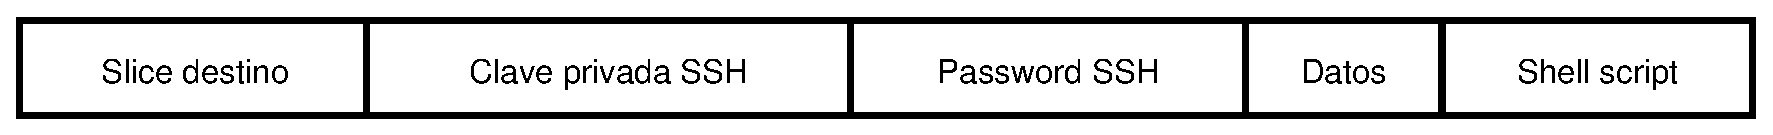
\includegraphics[scale=0.5]{paq_-_uplfs-pldb.eps}
	\caption{Paquete gen�rico \uplfs $\rightarrow$ \dplc}
	\label{fig:paq_-_uplfs-pldb}
\end{figure}


\subsubsection{Datos}
% TODO: En caso de que el paquete contenga el campo \texttt{Cmd}.....

\begin{figure}[h]
	\centering
	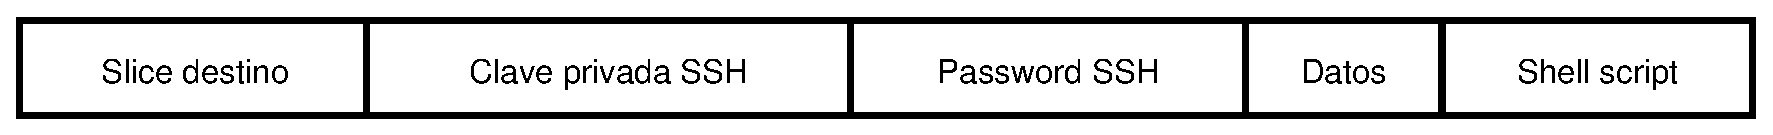
\includegraphics[scale=0.5]{paq_-_uplfs-pldb_-_data.eps}
	\caption{Paquete de datos \uplfs $\rightarrow$ \dplc}
	\label{fig:paq_-_uplfs-pldb_-_data}
\end{figure}

% TODO: Datos => lista ficheros + ficheros?
%       (kernel permite agrupaci�n de ficheros en un env�o?)
% TODO: si ya se pre-acredita, no hace falta ahora enviar passwd+clave
% TODO: otros tipos de paquete?

\begin{description}
	\item[Slice destino:] nombre del slice destino al que va destinado el
		paquete

	\item[Clave/Password privados ssh:] clave y password privados de ssh
para
		que	\dplc se comunique con el slice destino

	\item[Datos:] datos a desplegar en el slice destino

	\item[Shell script:] shell script a ejecutar una vez desplegados los
		ficheros (optativo)
\end{description}


\subsubsection{Registro de oyente}

% TODO Formate de paquete de registro



\section{\dplc $\rightarrow$ \dpld}
\label{sect:warnings}

Los nodos \dplc deben informar de los cambios en los grupos slice destino
a los \dpld que est�n registrados en ellos para esos slice.

Los cambios pueden ser:
\begin{itemize}
	\item Se a�ade un nuevo nodo al slice.

	\item Se quita un nodo del slice.

	\item Modificaci�n de ficheros (invalidaci�n).

	\item Se requiere autentificaci�n.
\end{itemize}

Para anunciar estos cambios hemos dise�ado un paquete de warning mediante el
cual los nodos \dplc los anuncian a los \dpld registrados.

%TODO figura paquete warning
Campo 1: tipo de cambio.
Campo 2: string (nodo o fichero).
Campo 3: shared o unshared
...

Para autentificar los paquetes de warning se firman con la clave privada
de \dplc.


\chapter{Caminos de operaci�n}

\textbf{\textit{En este cap�tulo comentaremos los diagramas de secuencia que
seguir�an las comunicaciones entre los componentes para tener una idea general
del sistema de modo visual.}}



\section{Listado de nodos}

El comando que lanzar�a esta operaci�n seria \texttt{ls /plfs/nodes/}, y el
diagrama de sus operaciones es el que se muestra en la figura
\ref{fig:act_-_ls_nodes}.

\begin{figure}[h]
	\centering
	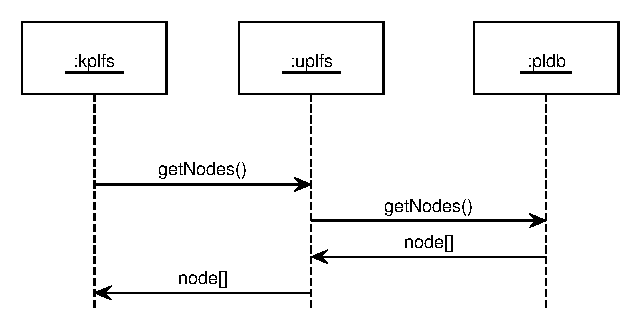
\includegraphics[scale=1.0]{act_-_ls_nodes.eps}
	\caption{Listado de nodos}
	\label{fig:act_-_ls_nodes}
\end{figure}



\section{Listado de slices}

El comando que lanzar�a esta operaci�n seria \texttt{ls /plfs/slices/}, y el
diagrama de sus operaciones es el que se muestra en la figura
\ref{fig:act_-_ls_slices}.

\begin{figure}[h]
	\centering
	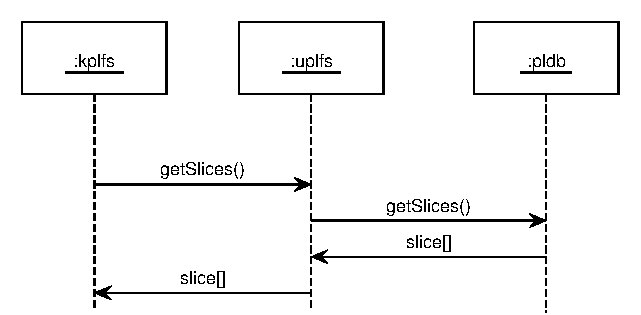
\includegraphics[scale=1.0]{act_-_ls_slices.eps}
	\caption{Listado de slices}
	\label{fig:act_-_ls_slices}
\end{figure}



\section{Listado de ficheros compartidos}

El comando que lanzar�a esta operaci�n ser�a \texttt{ls
/plfs/slices/\textless{}slice\textgreater/shared/}, y el diagrama de sus
operaciones es el que se muestra en la figura \ref{fig:act_-_ls_shared}.

\begin{figure}[h]
	\centering
	\includegraphics[scale=1.0]{act_-_ls_shared.eps}
	\caption{Listado de ficheros compartidos}
	\label{fig:act_-_ls_shared}
\end{figure}



\section{Listado de nodos de un slice}

El comando que lanzar�a esta operaci�n ser�a \texttt{ls
/plfs/slices/\textless{}slice\textgreater/nodes/}, y el diagrama de sus
operaciones es el que se muestra en la figura \ref{fig:act_-_ls_slice_nodes}.

\begin{figure}[h]
	\centering
	\includegraphics[scale=1.0]{act_-_ls_slice_nodes.eps}
	\caption{Listado de nodos de un slice}
	\label{fig:act_-_ls_slice_nodes}
\end{figure}



\section{Listado de ficheros no compartidos}

El comando que lanzar�a esta operaci�n ser�a \texttt{ls
/plfs/slices/\textless{}slice\textgreater/nodes/\textless{}node\textgreater/unshared/},
y el diagrama de sus operaciones es el que se muestra en la figura
\ref{fig:act_-_ls_unshared}.

\begin{figure}[h]
	\centering
	\includegraphics[scale=1.0]{act_-_ls_unshared.eps}
	\caption{Listado de ficheros no compartidos}
	\label{fig:act_-_ls_unshared}
\end{figure}



\section{Obtenci�n de un fichero}

El comando que lanzar�a esta operaci�n ser�a, por ejemplo, un \texttt{cat} de
un fichero, ya fuera en \texttt{shared} o \texttt{unshared}, y el diagrama de
sus operaciones es el que se muestra en la figura \ref{fig:act_-_get}.

\begin{figure}[h]
	\centering
	\includegraphics[scale=1.0]{act_-_get.eps}
	\caption{Obtenci�n de un fichero}
	\label{fig:act_-_get}
\end{figure}



\section{Desplegamiento}

% TODO: desplegar el soft de desplegamiento si no esta presente y es un nuevo
% nodo?

El comando que lanzar�a esta operaci�n ser�a, por ejemplo, un \texttt{cp} de
un fichero, ya fuera a \texttt{shared} a \texttt{unshared}, y el diagrama de
sus operaciones es el que se muestra en la figura \ref{fig:act_-_put}.

\begin{figure}[h]
	\centering
	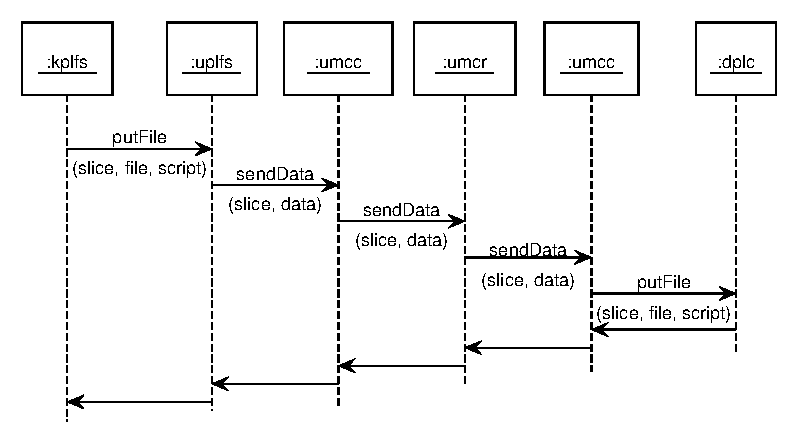
\includegraphics[scale=1.0]{act_-_put.eps}
	\caption{Desplegamiento}
	\label{fig:act_-_put}
\end{figure}



\section{Adici�n de un nodo a un grupo}

�sta operaci�n se llevar�a a cabo al crear una nueva m�quina virtual en un
nodo donde ya este corriendo \dplc, y el diagrama de sus operaciones es el que
se muestra en la figura \ref{fig:act_-_join}.

\begin{figure}[h]
	\centering
	\includegraphics[scale=1.0]{act_-_join.eps}
	\caption{Adici�n de un nodo a un grupo}
	\label{fig:act_-_join}
\end{figure}



\section{Eliminaci�n de un nodo de un grupo}

�sta operaci�n se llevar�a a cabo al eliminar una m�quina virtual de un nodo
donde ya este corriendo \dplc, y el diagrama de sus operaciones es el que se
muestra en la figura \ref{fig:act_-_delete}.

\begin{figure}[h]
	\centering
	\includegraphics[scale=1.0]{act_-_delete.eps}
	\caption{Eliminaci�n de un nodo de un grupo}
	\label{fig:act_-_delete}
\end{figure}



\pagebreak
\addcontentsline{toc}{chapter}{Bibliograf�a}
\bibliographystyle{plain}
\bibliography{00-plfs}

\end{document}

